\documentclass[oneside,11pt,openright]{report}

\usepackage[latin1]{inputenc}
\usepackage[american]{babel}
\usepackage{a4}
\usepackage{latexsym}
\usepackage{amssymb}
\usepackage{amsmath}
\usepackage{epsfig}
\usepackage[T1]{fontenc}
\usepackage{lmodern}
\usepackage[labeled]{multibib}
\usepackage{color}
\usepackage{datetime}
\usepackage{epstopdf} 

\usepackage{pgf,tikz}
\usepackage{comment}
\usetikzlibrary{arrows,automata}
\usetikzlibrary{backgrounds,fit}
\usetikzlibrary{shapes,patterns}
\usetikzlibrary{calc,chains,positioning}

\renewcommand*\ttdefault{txtt}
\newcommand{\BigO}[1]{\ensuremath{\operatorname{O}\left(#1\right)}}
\newcommand{\BigT}[1]{\ensuremath{\Theta\left(#1\right)}}
\newcommand{\specialcell}[2][c]{%
  \begin{tabular}[#1]{@{}c@{}}#2\end{tabular}}
% see http://imf.au.dk/system/latex/bog/

\newcommand{\DeleteMin}{\textsc{DeleteMin}}
\newcommand{\DecreaseKey}{\textsc{DecreaseKey}}
\newcommand{\Delete}{\textsc{Delete}}
\newcommand{\Insert}{\textsc{Insert}}

\begin{document}

%%%%%%%%%%%%%%%%%%%%%%%%%%%%%%%%%%%%%%%%%%%%%%%%%%%%%%%%%%%%%%%%%%%%%%%

\pagestyle{empty} 
\pagenumbering{roman} 
\vspace*{\fill}\noindent{\rule{\linewidth}{1mm}\\[4ex]
{\Huge\sf Binary Heaps, Fibonacci Heaps and\\[2ex]Dijkstras shortest path}\\[4ex]
{\huge\sf Kristoffer Just Andersen, 20051234\\[2ex]
\huge\sf Troels Leth Jensen, 20051234 \\[2ex]
\huge\sf Morten Krogh-Jespersen, 20022362}\\[2ex]
\noindent\rule{\linewidth}{1mm}\\[4ex]
\noindent{\Large\sf Project 1, Advanced Data Structures 2013, Computer Science\\[1ex] 
\monthname\ \the\year  \\[1ex] Advisor: Gerth St�lting Brodal\\[15ex]}\\[\fill]}

\epsfig{file=logo.eps}\clearpage

%%%%%%%%%%%%%%%%%%%%%%%%%%%%%%%%%%%%%%%%%%%%%%%%%%%%%%%%%%%%%%%%%%%%%%%

\tableofcontents
\pagenumbering{arabic}
\setcounter{secnumdepth}{2}

%%%%%%%%%%%%%%%%%%%%%%%%%%%%%%%%%%%%%%%%%%%%%%%%%%%%%%%%%%%%%%%%%%%%%%%

\chapter{Introduction}

needs content

\chapter{Binary heaps}

needs content

\section{Binary heap with array}

needs content

\section{Implementing decrease key}

needs content

\section{Time-complexity for binary heap with array}

\section{Binary heap with pointers}

needs content

\section{Implementing decrease key}

needs content

\section{Time-complexity for binary heap with pointers}

\section{Testing correctness of Binary Heaps}

needs content

\chapter{Fibonacci heaps}

In this chapter we focus on Fibonacci heaps, which is a data structure that has a forest of rooted trees as opposed to a binary heap that only has one tree \cite{FT87}. The data structure was invented by Michael L. Fredman and Robert Endre Tarjan and was published in the Journal of ACM in 1987. It has it name because the size of any subtree in a Fibonacci heap will be lower bounded by $F_{k+2}$ where $k$ is the degree of the root in that subtree and $F$ is the Fibonacci function. Below is the time-complexities of each of the heap operations listed:

\begin{center}
  \begin{tabular}{ l | c | c | c }
    Operation & Binary heap & \specialcell{Fibonacci heap v1\\(amortized)} & \specialcell{Fibonacci heap v2\\(amortized)} \\ \hline
    MakeHeap & $\BigT{1}$ & $\BigT{1}$ & $\BigT{1}$ \\ 
    FindMin & $\BigT{1}$ & $\BigT{1}$ & $\BigO{l(\lg (\frac{n}{l}) + 1)}$\\ 
    Insert & $\BigT{\lg n}$ & $\BigT{1}$ & $\BigT{1}$ \\ 
    DeleteMin & $\BigT{\lg n}$ & $\BigO{\lg n}$ & $\BigT{1}$  \\ 
    DecreaseKey & $\BigT{\lg n}$ & $\BigO{1}$ & $\BigO{1}$ \\ 
    Delete & $\BigT{\lg n}$ & $\BigO{\lg n}$ & $\BigT{1}$ \\ 
    Meld & $\BigT{n}$ & $\BigT{1}$ & $\BigT{1}$ \\
  \end{tabular}
\end{center}

\section{Fibonacci heap version 1}

The first Fibonacci heap variant we present is the original version proposed in FT87. A potential function is used to analyze the perfomance, thus the above stated time-complexities are amortized.

Our implementation pretty much follows from the article, with few exceptions. The article do not specify exactly how a node is found from an item in constant time, so we decided to place a pointer on the item. Melding is not totally destructable since we join the heap in of the two existing heaps and return an arbitrary one. 

The article mentions that $\Delete$ takes $\BigO{1}$ if the node to remove is not the min-node and without cascading deletes. The children of the node to delete must be moved up onto the root which can only be done in constant time if every children has a pointer to a parent pointer. In this way, we only have to change one pointer to update all parent pointers for the children of the beforementioned node. Since the running time of the algorithm is amortized $\BigO{\lg n}$ we chose a simpler version where we just update all parent pointers.


\section{Worst case time-complexity for Fib heap v1}

There are three operations where changes to the potential occurs, and thus, the stated times are amortized for $\DeleteMin$, $\DecreaseKey$ and $\Delete$. Below we illustrate the worst-case for each of these operations by showing a configuration and how that configuration can be obtained from a sequence of operations :

\subsection{Worst case time-complexity for $\DeleteMin$}

The worst configuration for $\DeleteMin$ is when all the nodes in the heap is at the root in a linked list:

\begin{center}
  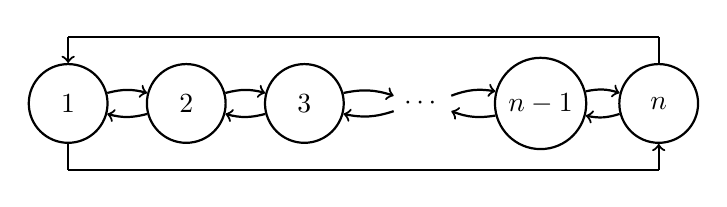
\begin{tikzpicture}[thick,->,auto,node distance=1.5cm]
    \tikzstyle{state}=[circle, minimum size=1cm, draw]
  
    \node[state]    	  (1) {1};
    \node[state]         (2) [right of=1] {2};
    \node[state]         (3) [right of=2] {3};
    \node          (dots) [right of=3] {$\cdots$};
    \node[state]         (nminusone) [right of=dots] {$n-1$};
    \node[state]         (n) [right of=nminusone] {$n$};
    \node          (dummy1) [below=0.2cm of 1] {};
    \node          (dummy2) [below=0.2cm of n] {};
    \node          (dummy3) [above=0.2cm of 1] {};
    \node          (dummy4) [above=0.2cm of n] {};
    
    \path (1)   edge [bend left=15] (2);
    \path (2) edge [bend left=15] (1);
    \path (2) edge [bend left=15] (3);
    \path (3) edge [bend left=15] (2);
    \path (3) edge [bend left=15] (dots);
    \path (dots) edge [bend left=15] (3);
    \path (dots) edge [bend left=15] (nminusone);
    \path (nminusone) edge [bend left=15] (dots);
    \path (nminusone) edge [bend left=15] (n);
    \path (n) edge [bend left=15] (nminusone);
    \path[-] (1) edge (dummy1.center);
    \path[-] (dummy1.center) edge (dummy2.center);
    \path (dummy2.center) edge (n);
    \path[-] (n) edge (dummy4.center);
    \path[-] (dummy4.center) edge (dummy3.center);
    \path (dummy3.center) edge (1);
  \end{tikzpicture}
\end{center}

This configuration can be achievede by just calling insert $n$ times. For simplicity, let us assume that $n$ is odd, and a call to $\DeleteMin$ happens. In the above example 1 will be removed and we are left with $n-1$ root nodes to link. This results in $n-1$ key comparisons, but all the trees of rank 1 will be joined too and this will continue until no trees of duplicate size is found.
\begin{align*}
  \text{\# of operations} = \BigO{n-1} + \BigO{\frac{n-1}{2}} + \BigO{\frac{n-1}{2^2}} + \cdots + \BigO{\frac{n-1}{2^{\lg (n-1)-1}}}
\end{align*}

which is $\BigT{n}$.

\subsection{Worst case time-complexity for $\Delete$ and $\DecreaseKey$}

If $\Delete$ is invoked with the min-node as argument then $\Delete$ calls $\DeleteMin$, therefore, the worst case for $\Delete$ is $\BigT{n}$, but we will show that without the min-node as argument, we still end up with $\BigT{n}$.

If we delete a child to an arbitrary node $x$ we mark $x$ if is not marked and if it is marked, we cut $x$ from its parent, move the subtree formed by $x$ to the root and try to mark the previous parent of $x$. This could result in cascading deletes. Therefore, the worst situation would be the following configuration:
\begin{center}
  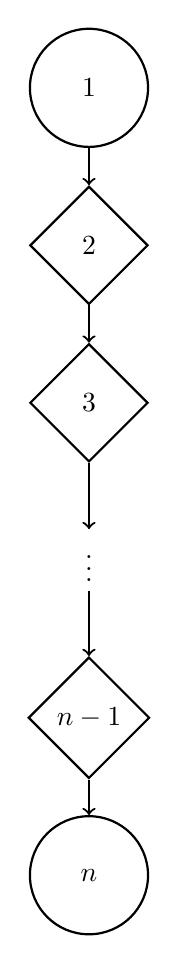
\begin{tikzpicture}[thick,->,auto,node distance=2cm]
    \tikzstyle{node}=[circle, minimum size=1.5cm, draw]
    \tikzstyle{marked}=[diamond, minimum size=1.5cm, draw]
  
    \node[node]    	  (1) {1};
    \node[marked]         (2) [below of=1] {2};
    \node[marked]         (3) [below of=2] {3};
    \node          (dots) [below of=3] {$\vdots$};
    \node[marked]         (nminusone) [below of=dots] {$n-1$};
    \node[node]         (n) [below of=nminusone] {$n$};
    
    \path (1) edge (2);
    \path (2) edge (3);
    \path (3) edge (dots);
    \path (dots) edge (nminusone);
    \path (nminusone) edge (n);

  \end{tikzpicture}
\end{center}

where a diamond is modelling a marked node. If either $\DecreaseKey$ or $\Delete$ is called with an item corresponding to node $n$ a cascading delete will begin and will not stop until it reaches $2$ in this example. The amount of operations is therefore the entire chain:
\begin{align*}
  \text{length of chain} = n - 1
\end{align*}

which is $\BigT{n}$.

Such a configuration can be obtained by calling $\Insert$ with two very high numbers $x$ and $y$ and one smaller and call $\DeleteMin$:

\begin{center}
  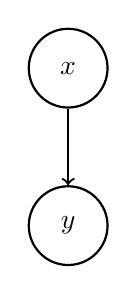
\begin{tikzpicture}[thick,->,auto,node distance=2cm]
    \tikzstyle{node}=[circle, minimum size=1cm, draw]
    \tikzstyle{marked}=[diamond, minimum size=1cm, draw]
  
    \node[node]    	  (1) {$x$};
    \node[node]           (2) [below of=1] {$y$};
    
    \path (1) edge (2);

  \end{tikzpicture}
\end{center}

If we insert three new items $x'$, $y'$ $z$ with keys slightly smaller where $z$ is the smallest key we will have the following forest:

\begin{center}
  \begin{tikzpicture}[thick,->,auto,node distance=2cm]
    \tikzstyle{node}=[circle, minimum size=1cm, draw]
  
    \node[node]    	  (x) {$x$};
    \node[node]           (y) [below of=x] {$y$};
    \node[node]    	  (x') [right of=x] {$x'$};
    \node[node]    	  (y') [right of=x'] {$y'$}; 
    \node[node]    	  (z) [right of=y'] {$z$};
   
    \path (1) edge (2);

  \end{tikzpicture}
\end{center}

If we call $\DeleteMin$ and call insert with three new items, we can get the following configuration:

\begin{center}
  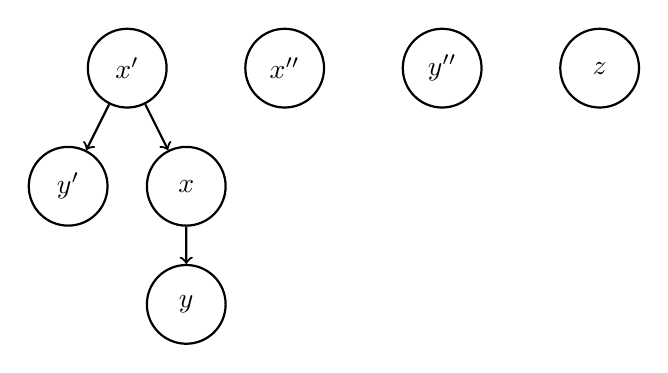
\begin{tikzpicture}[thick,->,auto,node distance=2cm]
    \tikzstyle{node}=[circle, minimum size=1cm, draw]
  
    \node[node]    	  (x') {$x'$}
    child{node[node]      (y') {$y'$}}
    child{node[node]      (x) {$x$}
      child{node[node]    (y) {$y$}}};
    \node[node]    	  (x'') [right of=x'] {$x''$};
    \node[node]    	  (y'') [right of=x''] {$y''$}; 
    \node[node]    	  (z) [right of=y''] {$z$};
   
  \end{tikzpicture}
\end{center}

where $z$ again is the smallest key. We can $\Delete$ $y'$ and call $\DeleteMin$, which now gives:

\begin{center}
  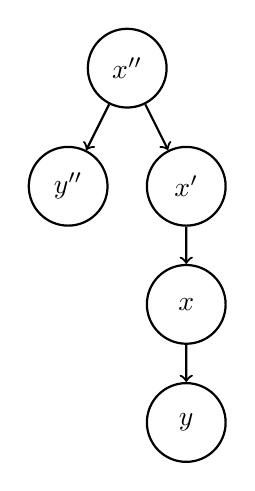
\begin{tikzpicture}[thick,->,auto,node distance=2cm]
    \tikzstyle{node}=[circle, minimum size=1cm, draw]
  
    \node[node]    	  (x'') {$x''$}
    child{node[node]      (y'') {$y''$}}
    child{node[node]      (x') {$x'$}
      child{node[node]    (x) {$x$}
        child{node[node]  (y) {$y$}}}};
   
  \end{tikzpicture}
\end{center}

By using this approach we can easily build up a single chain of height $n$.

\section{Fibonacci heap version 2}

needs content

\section{Worst case time-complexity for Fib heap v2}

needs content

\section{Testing correctness of Fibonacci Heaps}

needs content

\chapter{Test-results}

needs content

\chapter{Dijkstra}

needs content

\chapter{Binary heap vs Fibonacci heap}

needs content

\chapter{Test-results}

needs content

\chapter{Conlusion}

needs contents


%%%%%%%%%%%%%%%%%%%%%%%%%%%%%%%%%%%%%%%%%%%%%%%%%%%%%%%%%%%%%%%%%%%%%%%

\addcontentsline{toc}{chapter}{Bibliography}
\bibliographystyle{plain} 
\bibliography{report}

\end{document}

